% Created 2024-10-20 So 14:41
% Intended LaTeX compiler: pdflatex
\documentclass[11pt]{article}
\usepackage[utf8]{inputenc}
\usepackage[T1]{fontenc}
\usepackage{graphicx}
\usepackage{longtable}
\usepackage{wrapfig}
\usepackage{rotating}
\usepackage[normalem]{ulem}
\usepackage{amsmath}
\usepackage{amssymb}
\usepackage{capt-of}
\usepackage{hyperref}
\usepackage{songs_of_maya}
\usepackage[a5paper, total={128mm, 190mm}]{geometry}
\setcounter{secnumdepth}{3}
\date{}
\title{Songs of Maya}
\hypersetup{
 pdfauthor={Lukas Zumvorde},
 pdftitle={Songs of Maya},
 pdfkeywords={},
 pdfsubject={},
 pdfcreator={Emacs 29.4 (Org mode 9.7.9)}, 
 pdflang={English}}
\begin{document}

\maketitle
\tableofcontents

{\rowcolors{1}{grey!20}{grey!10}

\newpage
\section{Introduction}
\label{sec:org04ee2ce}

Songs of Maya is a generic, light, and abstract role playing rule set with a focus on keeping the game balanced while maintaining an even probalibity distribution and promoting creative story telling. It leans towards a cinematic play style.
\subsection{Goals}
\label{sec:org23a109f}

\begin{itemize}
\item Rules light
\item Flexible
\item World agnostic
\item Consistent probability distribution
\item Easy game preparation
\item Little bookkeeping during the game
\end{itemize}
\subsection{Inspirations}
\label{sec:org688b12a}

This game did not come from nothing. Many other games had an impact on its creation. Some of the most impactfull ones are the following.:

This games systems for aspects and movement were heavily inspired from the Fate Core system.
Karma was originally inspired by Fate Cores Fate Points, but EZD6 had the better name for the concept.
The distribution of attributes into categories was inspired by the AERA RPG.
The fate die to create unexpected events was inspired by the One Page Solo RPG Engine.
The optional rule "Only Players Roll" is taken from the Cypher System.
The turn order was taken from Tides of Ambition.
\subsection{How to use the game}
\label{sec:org0d58259}

First rule of Gaming: Have fun. If the rules hinder you from having fun then screw the rules.

Second rule of Gaming: When in doubt use common sense. The rules will never be perfect. If something is illogical when using the rules or if no rules exists for the situation then feel free to find your own. 

Third rule of Gaming: Use the aspects value as a guideline and be creative with what it could mean. Does a flame wall having a value of 4 mean that it has a difficulty of 4 to jump over it or does it attack anyone jumping over with 4 dice? Do what fits your story. 
\subsection{Conventions}
\label{sec:org893852d}
\textbf{Dice shorthand}: \(3 d 6\) means rolling three six sided dice and summing up the results. \(1 d_0 2\) means rolling 1 dice whose sides go from 0 to 2 (three sides in total). \(2 \times d_0 8\) means rolling a dice whose sides go from 0 to 8 and multiplying the result by 2.

\textbf{Aspects}: Aspects are highlighted like this \aspect{example aspect 3}. The tailing number indicates the value of the aspect. If an aspect has an additional number in square brackets (\aspect{example aspect 2[4]}), this denotes the \hyperref[sec:org674d41e]{resistance} of the aspect. 

\textbf{Quick Reference}: All core rules can be found in \texttt{Quick Reference} blocks at the beginning of their respective sections. Everything else are just explainations and extensions of these rules.
\section{Rules}
\label{sec:org112b32c}

\subsection{Dice Mechanics}
\label{sec:org4a0f369}
\begin{short}
The dice points (DP) are calculated from the attributes and aspects. They are used to buy the dice you roll for a check.

\begin{itemize}
\item A die is worth exactly its average result in DP
\begin{itemize}
\item \(1 d N\) is worth \(\frac{N+1}{2}\) DP
\item \(1 d_0 N\) is worth \(\frac{N}{2}\) DP
\item Throwing a N sided die twice and subtracting the lower result from the higher is worth \(\frac{N}{3}\) DP
\end{itemize}
\item It is possible for costs to contain a fraction of a DP.
\item A constant \(N\) are worth \(N\) dice points (generally you should limit this to \(\frac{1}{4}\) of the dice points). Fractions of a point are possible.
\item Any dice multiplied by a factor \(F\) is worth the price of a single die multiplied by this factor \(F\)
\end{itemize}

You can decide for each check individualy what dice to roll, It is still advisable to always use the same dice if possible. 
\end{short}

To keep all possible results evenly distributed you should favor to roll just a single die, that has as at least 6 sides. Since many 10 sided dice go from 0 to 9 (\(d_0 9\)) they are a good default (cost \(4.5\) DP). Pick higher factors (\(F \times d_0 9\)) if you have significantly more DP available. Dont be afraid of the fractional DP costs. 

There are multiple ways to simulate \(d_0 N\) dice. To simulate a \ldots{}
\begin{itemize}
\item \(d_0 2\): take a \(d6\) and count 1,2 as 0; 3,4 as 1; and 5,6 as 2.
\item \(d_0 2\): roll a fudge die (also known as fate dice). Count the empty sides as 0, count the "-" as 1 and "+" as 2. (essentially counting the number of lines.)
\item \(d_0 8\): roll a \(d10\) (most actually go from 0 to 9). Reroll the die if you roll a 9.
\item \(d_0 N\) with \(N \le 12\): Take a deck of cards. Count the queen as 0, ace as 1, numbers as they are, joker as 11, and king as 12. Discard any cards you dont need.
\end{itemize}

Sometimes it makes no sense to roll dice, but we want a constant value. Then we can \hyperref[sec:org386b63b]{take the average}. This means instead of rolling dice we just take the dice points as if it were the result of a roll. This is fair since it is also the average result of a roll.

\begin{center}
\begin{tabular}{lr}
Dice & Cost (DP)\\
\hline
\(d3\) & 2\\
\(d4\) & 2.5\\
\(d6\) & 3.5\\
\(d8\) & 4.5\\
\(d10\) & 5.5\\
\(d12\) & 6.5\\
\(d20\) & 10.5\\
\(d_0 2\) & 1\\
\(d_0 8\) & 4\\
\(d_0 9\) & 4.5\\
\(d_0 12\) & 6\\
\end{tabular}
\end{center}
\subsection{Attributes}
\label{sec:orgb96d653}
\begin{short}
There are the 8 attributes Strength, Dexterity, Will, Intellect, Empathy, Charisma, Gear, and Finances. Each attribute gets a whole number value.
\end{short}

Attributes describe a characters potential. The higher the value the greater things a character can achieve. There are the following 8 Attributes belonging to the 4 categories.

\begin{center}
\begin{tabular}{lll}
\textbf{Category} & \textbf{Attribute} & \textbf{Description}\\
\hline
Physical & Strength & strength and hardiness\\
 & Dexterity & agility, speed, precision\\
\hline
Mental & Will & perseverance, attention\\
 & Intellect & intelligence, knowledge\\
\hline
Social & Empathy & understanding people\\
 & Charisma & interacting with people\\
\hline
Resources & Gear & Gear you have prepared\\
 & Finances & Money and investments\\
\end{tabular}
\end{center}

The attributes value is the basis for the dice points one has available for \hyperref[sec:org6437075]{checks}. 
\subsection{Aspects}
\label{sec:org43144d2}
\begin{short}
Aspects have a descriptive name and a whole number value called its aspect points (AP).
\begin{itemize}
\item Create: Make a check. The resulting AP are the AP of the new aspect.
\item Use: Add the AP of the aspect to the check. Any AP can only be used once per round.
\item Multiple Targets: To create an aspect that effects an area or multiple targets half the AP.
\item Duration: By default an aspect can be used once. To make it apply every round until the duration is over, half the AP.
\item Acting: Aspects can perform actions on their own. For this use the AP as the dice points.
\item Remove: To remove an aspect you need to make a check. Reduce the AP of the aspect by the AP of the check.
\item Resistance: Aspects can resist being removed. To reduce the AP of the check for removal by 1 for each resistance point. A point of resistance costs 1 AP.
\end{itemize}
\end{short}


Aspects are a combination of a descriptors and a value. When invoked the aspects value is added or subtracted from the dice points  for \hyperref[sec:org6437075]{checks}. An aspect is always bound to something. Be it a player, a NPC, an object or even a zone. Be creative with aspects. Try to bind their effects to the value and they should stay balanced enough.
\paragraph*{Creating an Aspect}
\label{sec:org4930be3}

An aspect can be created at any time by the GM. It can also be created by any player, NPC or even object. To create an aspect all but the GM need to make a check. The aspect points (AP) from this check can be used to create an aspect. Increasing or decreasing an aspects value by 1 costs 1 AP (aspect point). The description of the aspect can be decided freely. 

\begin{pwexample}
Arthur the mage wants to inflame the grass around him to channel the enemies into a one on one battle with his Companions. The GM likes this idea and creates the aspect \aspect{Dry Grass 1} that Arthur can use. Arthur decides to cast his spell, succeeds with 3 AP, and creates the aspect \aspect{Wall of Fire 3}. Now any enemy has to either go around the wall or get burned. If an enemy tires to jump through, they have to roll on it against the fires 3 dice. If the fire succeeds they get burned.
\end{pwexample}
\paragraph*{Using Aspects}
\label{sec:orgd29707c}

Whenever it makes narrative sense, an aspect can be used (also called invoked). When used an aspect adds its value to the number of points that can be used for a check. It is also possible to call out an aspect to be used to hinder a check. Then the value is subtracted from the points instead. An aspect can both be used for actions and reactions but never at the same time. If you use  aspects in a contest make sure that aspects are not used more than once per round by a character or their points are distributed over different actions.
\paragraph*{Multiple Targets or Area Aspects}
\label{sec:orgd2556ec}
An aspect can affect a zone or multiple individual targets. To create such an aspect costs double the AP (aspect points). Exceptions may be made by the GM. 
\paragraph*{Enduring Aspects}
\label{sec:orgcdb4f3f}
An aspect can be over within a round or it can last longer. Normally aspects last for a round or until invoked once. If your aspect should last longer and potentially apply each round it should cost double the AP (aspect points) for each increase. Exceptions may be made by the GM. In general it can be said, that an aspect lasts as long as it makes sense. It is possible to make aspects last even longer. Use the following table as an orientation.
\begin{center}
\begin{tabular}{ll}
Round & A few seconds or until used once, Example: triped\\
Scene & Until the end of a fight, Example: Frightened\\
Mission & Until the end of a story or quest, Example: Wounded\\
Campagne & Until the end of a story arc, Example: Demonic Poison\\
\end{tabular}
\end{center}
\paragraph*{Acting Aspects}
\label{sec:org812bc01}

Sometimes an aspect should perform actions on its own. Each round they can act like any other player or NPC. They use their value for their actions.

\begin{pwexample}
\aspect{Poison Cloud 2}: Each round it tries to use 2 dice to poison any inside. Since it impacts a zone it can do this for everyone inside the zone every round.
\end{pwexample}
\paragraph*{Resistant Aspects}
\label{sec:org674d41e}
An aspect can have resistance to being removed. The resistance is subtracted from any attempt to remove this aspect. Each point of resistance costs 1 AP. Be creative when invoking a resistant aspect. For example armor could be implemented as an aspect with resistance.

\begin{pwexample}
A heavy door blocks the way. The GM creates the aspect \aspect{Fortified Door 5[2]}. This means the aspect has a value of 5 with a resistance of 2. The players try to break through with pure strength. On their first try they get 4 AP. 2 get absorbed by the doors resistance and the rest weakens the door. The doors aspect is now \aspect{Fortified Door 3[2]}. On their second try the players get 6 AP and break through.
If the players had decided to pick the lock the GM may had ignored the resistance value.
\end{pwexample}
\paragraph*{Character Aspects}
\label{sec:orgfb4b311}

Aspects can also be bound to a character and be bought with CP (character points). If an aspect is mostly negative in nature it may give you CP instead. Character aspects can be invoked by the GM to make the character do something. 
\paragraph*{Damage}
\label{sec:orgb098020}

Aspects are also used to represent damage a character or object has taken. If a character is unable to act in a scene because too many aspects hinder him, it is a good idea to narrate them out of the scene. It is also a good time to create a fitting negative character aspect representing this loss (like \aspect{lost an arm} or \aspect{fear of water} or \aspect{hateful of orcs}).
\paragraph*{Converting Aspects}
\label{sec:orgef00708}

Sometimes it may be usefull to change one or more aspects into another. In those cases just create a new aspects for an equivalent number of AP as all the aspects you remove for it.
A good example for this is replacing a more abstract \aspect{combat damage} at the end of a fight, with a more permanent and more interesting long term damage.

\begin{pwexample}
During a fist fight against the goblin chief the glorious knight has taken 7 damage. After he lost the fight this gets converted into the more enduring aspect \aspect{wounded pride 3}. 
\end{pwexample}
\subsection{Checks}
\label{sec:org6437075}
\begin{short}
Add points of attribute and aspects to get the dice points. Roll one or multiple dice that are equvalent to the dice points in value. The result of the roll are the aspect points (AP) of the check.
\begin{itemize}
\item Difficulty: Some aspects hinder a check. For them consider the AP to be negative instead.
\item Collaboration: Add either the dice points for the checks or the AP of all checks made together.
\item Risky: Roll an additional \(d6\). If it shows a \(6\) then use the result of the check to create a negative aspect instead.
\item Take Time: Make multiple checks and add the AP.
\end{itemize}
\end{short}

Checks are rolled when the outcome of an action is not certain. Each check is bound to an \hyperref[sec:orgb96d653]{attribute}.

Add the points in the relevant attribute and all applicable \hyperref[sec:org43144d2]{aspects} together. These are your dice points. You get the result of the roll in aspect points (AP) to create or change an Aspect.

If the aspect points are zero or negative the check fails.

If the aspect points are not a whole number, then you can round the result just before creating the aspect.
\paragraph*{Difficulty}
\label{sec:org9123948}
The checks difficulty is the sum of all aspects that are to be overcome or created. This means that a door having the difficulty 3 to be opened is the same thing as the door having the aspect \aspect{Closed 3} on it. If an obstacle can not be partially overcome you can give it a \hyperref[sec:org674d41e]{resistant aspect}.

\begin{pwexample}
The player tries to pick a door lock. The GM decides that he can not partially pick a lock and thus chip away at the door. So he gives it the aspect \aspect{closed 1[5]}. This means that the player needs at least 6 AP to open it and has to do it with one check.
\end{pwexample}
\paragraph*{Collaborative checks}
\label{sec:org38b2b58}
Everyone rolls individually and then sum together all AP. Alternatively you can also sum up the DP and make a single roll.
\paragraph*{Risky checks}
\label{sec:orgdb86fca}
Roll the same dice you rolled for the check again. If these show a higher value then it comes to a bad outcome. The original check dice (not those for the risk check) are used to create a negative aspect.

The chance of something bad happening is quite high (around 50\%) unless you reduce the risk. If this is too risky for your game then you can require two risk rolls instead. Something bad only happens if both risk rolls are higher (around 30\%). 

Before the check a player can reduce or heighten the risk. For this select a number. For the comparison of the dice, the check roll is increased by the number, but for the result the check is decreased by the number. The check roll can not go below its regular minimum. Calculating the AP from the check happens after all this.
\paragraph*{Taking Time}
\label{sec:org1b8816a}
Sometimes a check is to difficult to achieve something within 1 check. Then it may be possible to do multiple checks over a longer time to accumulate the points needed. However, you must decide beforehand how many checks you want to take. The AP of all checks are accumulated after considering the difficulty. The GM has a veto right and can limit the amount of checks.
\paragraph*{Limited Aspects}
\label{sec:org4360fdd}
To prevent players from stacking up aspects endlessly it may be good to limit the ammount of points one can use. The dice points should be limited to double the sum of the relevant attribute and all used aspect points from chracter inherent aspects. Feel free to disregard this rule however if it does not fit well with the story.
\paragraph*{Multiple Checks}
\label{sec:orgf7661d4}
Sometimes the players fail to pass an obstacle with just one check. If the players have a new idea on how they might overcome the challenge then you can allow them another check. The new idea may add the checks AP to the previous attempt or replace them, depending on the narrative.

\begin{pwexample}
The player has to climb up a cliff. The cliff has the aspect \aspect{sheer rock face 6[2]} At frist he tires to just climb. He rolls a 3 on his check. This does not suffice and because of the 2 resistance of the aspect he has only overcome 1 of the 6 AP, he needs. This is harder than expected and considering that he has already climbed some of the distance a failure may end in a fall. He pulls out some wedges from his pack and starts to use them to create some better holds. For this the GM allows a new check, which he gets 7 AP from. With those he just barely climbs the rest of the distance.
\end{pwexample}
\paragraph*{Take the average}
\label{sec:org386b63b}
In some situations it may be good idea not to roll any dice at all. In those cases you can just assume that the average result was rolled. This means that you get the \texttt{dice points} in \texttt{AP} out of the check. 
\subsection{Contest}
\label{sec:org253cc89}
\begin{short}
Each participant can make one or more checks each round.
\begin{itemize}
\item Action: A check to create an aspect
\item Reaction: A check to prevent an aspect from being created.
\item Turn Order: Groups act together. If a groups surprises the other or has significantly fewer members they go first. Characters can act on their turn or at any later time in the round. When in doupt the players or the stronger go first.
\item Multiple (re)actions: Total number of points (dice points) gained from the attributes is the largest attribute value of all used in the checks. From each attribute (and aspect) you can use at most its value in points.
\end{itemize}
\end{short}

The prototypical contest is combat, but the same rules can be used any scenario where multiple parties act in opposition to each other. Be it a diplomatic debate or the hostile takeover of a company. 

A contest is divided into rounds. Each participant in the contest can make one or more checks each round. When it is a participants turn or on any later point in the round they can perform an action.
\paragraph*{Actions}
\label{sec:org18eefe4}
An action is a check that tries to create an aspect. Any kind of aspect can be created, based on what fits the scene. You can try to gain an advantageous position, or start a big fire.

The default aspect created in combat is \aspect{damage}. Damage is an \hyperref[sec:orgcdb4f3f]{enduring aspect} for the scene thus costing 2 AP per level of the aspect. After combat \aspect{damage} gets converted to one or more fitting negative aspects like \aspect{broken leg} or \aspect{battered and bruised}, These aspects are often times of a higher timeframe, therefore they cost more AP per level and are thus lower in effect.
If a character has more \aspect{damage} than he has points in an applicable attribute and character aspects combined then he is considered incapacitated for the rest of combat. This may mean that he is unconcious, writhing in pain or just to demoralised to fight.

Alternatively the aspect can be \aspect{stress} as a non enduring alernative to damage. \aspect{Stress} only holds for 1 round but cost only 1 AP per level of the aspect. It can be invoked to hinder the victims action. Note that you can only use any point of this aspect once in the round. 
\paragraph*{Reactions}
\label{sec:org3963c72}
Whenever someone takes an action and has rolled his dice anyone else can immediately try to perform a reaction to prevent it. A reaction does not by its nature create an aspect. If you announce this before the action is rolled you can take the average on a reaction. You have to announce the number of dice invested. The AP from the reaction are then subtracted from the AP of the action to lessen its effect.
\paragraph*{Turn Order}
\label{sec:orgf12a3c7}
\begin{itemize}
\item All characters of a group act together. The specific order within a group can be decided freely.
\item If a group surprises the others then they go first.
\item If a group has significantly fewer members, then they go first.
\item If all else fails determine the order randomly.
\end{itemize}

A character can act on his turn or at any later time in the round. If two characters wait for each other none of them can act.
\paragraph*{Multiple (re)actions}
\label{sec:orgec95a27}
Each round you can take multiple actions and reactions. The total number of points gained from the attributes is the largest attribute value of the checks. From each attribute you can use at most its value in DP in total. Each Aspect can only be used once per round or their AP (aspect points) have to be distributed to the (re)actions.
\paragraph*{Acting together}
\label{sec:org9280bf9}
When acting together all values are combined and a single combined check is made or alternatively everyone rolls seperately and only the AP are combined. To act together all have to act at the same time in the turn order, so effectively at the earliest when the slowest has his turn.
\subsection{Traits}
\label{sec:org24b0f9c}
\begin{short}
Traits allow characters to break rules in some way. Some checks that can only be performed because of a trait make those checks \hyperref[sec:orgdb86fca]{risky}. Traits can be bought for character points.
\end{short}

Traits are distinguishing things about the character that allow him to break a rule of the world or the game in some way. For example with the Trait Night Vision you can just see in the dark. No rolls required. Some traits (like all magic) should come with a risk, meaning all checks that can only be made with this trait are risky checks. Traits can be bought for character points, this is possible both at character creation and later in the game.

See the chapter \hyperref[sec:orgdba11b8]{List of Traits} for examples.
\subsection{Karma}
\label{sec:org8adc603}
\begin{short}
Each player can have up to 3 karma. They can be used at any point in time to repeat a single die roll (not just your own) or to add an interesting aspect to a scene. The GM has veto rights. Karma can be recovered by a characters aspect or trait being used against them or by objectively failing in a scene or as a reward for good role play, anything that brings joy to all players and the GM. 
\end{short}
\subsection{Character Creation}
\label{sec:orgd2f48eb}
\begin{short}
Distribute 150 CP on your Attributes, Aspects and Traits.

Use the rules under equipment to limit your starting gear.

Character Advancement:
You may reward your players with CP (character points) for reaching milestones in the story or simply surviving the session.

\begin{itemize}
\item An attribute point costs 6 CP.
\item An Aspect point typically costs 6 CP but can vary based on how specific they are.
\item A Trait typically costs 15 CP but can vary widely. Negative traits can even have a negative price.
\end{itemize}

A typical player character will have:
\begin{itemize}
\item all attributes with value 2 on average
\item 3 aspects with value 2
\item 1 trait
\end{itemize}
\end{short}
\subsection{Movement and Range}
\label{sec:org5281e6f}
\begin{short}
Sometimes it is useful to draw maps and define distances. In a contest split the area into roughly 3-5 zones. A character can move from one zone to another each round. If one can act at a range, like for example when shooting a bow, one can act 1-2 zones far. During the round a character is moving he can be considered to be in both zones at once.
\end{short}
\subsection{Items and Equipment}
\label{sec:orgb5d89a7}
\begin{short}
The RV of an item is the sum of all attached aspects AP. For multiple use items, remember that \hyperref[sec:orgcdb4f3f]{enduring aspects} cost double the AP.
\begin{itemize}
\item Equipment: Have gear with RV of up to the gear attribute in value. Have as much as you can carry or keep at home.
\item Buying: Make a finances check and have the RV+1 in AP. On success get the item and a negative aspect \aspect{Expences RV+1} on your finances for some time.
\item Crafting: Resources must be expended, worth RV-1. Make a check and have the RV in AP.
\item Gathering: Make a check against the RV.
\end{itemize}
\end{short}

Items are in essence just a named things with one or more attached aspects. The sum of the AP of all aspects on an item is its resource value (RV). For most items their apects are obvious and dont need to be mentioned specifically. For example if you use a sword with RV 4, then you can just assume that it has an aspect aiding in a fight for 2 points (because enduring aspects cost double). Some items may be \hyperref[sec:orgcdb4f3f]{enduring}, they can be used multiple times. Other items are a one use item like a first aid kit. 

\begin{center}
\begin{tabular}{c|l|l}
\textbf{RV} & \textbf{Description} & \textbf{Example}\\
\hline
0 & Free & a stick\\
2 & Cheap & simple clothes, basic tools\\
4 & Affordable & regular car, apartment\\
6 & Costly & regular house\\
8 & Expensive & sports car, designer clothes\\
10 & Very Expensive & small airplane\\
12 & Luxurious & private jet\\
\end{tabular}
\end{center}
\subsubsection{Equipment}
\label{sec:orge3732b0}
Characters can have gear with an individual value of up to the attribute Gear in RV on them. They must be able to carry all that gear on them or if it is part of their household it must fit in their normally furnished home. Apply reason as necessary.

When out adventuring characters have all the gear that they have written down. Additionally they can be allowed to make a Gear check against the RV of what they would like to have in the moment to see if they do. The check is risky and if they fail they get the negative aspect \aspect{Packed the wrong stuff} until the end of the mission or until they resupply.
\subsubsection{Buying}
\label{sec:orgeb36977}
Characters can buy new items with a Finances check. It works just like crafting an aspect with the resource value (RV) plus one, in aspect points (AP). If you succeed in buying the item then you take a negative aspect on your finances for some time. The GM does not have to let you retry on a fail. If you use items with aspects to do this like the \aspect{Treasure} you found during your last adventure you may lose them if you succeed on the check.
\subsubsection{Crafting}
\label{sec:org8bf4b6b}
Characters can also build their own items. For that they need the appropriate tools and resources. The resources may be bought and have a RV of the item to be build minus 1. To build the item the character needs to make a check and achieve at least the items RV in AP. If that fails the resources might be lost, depending on what they are.
\subsubsection{Gathering}
\label{sec:orgbce852e}
Resources can be gathered with a check and their RV as difficulty.
\section{Optional Rules}
\label{sec:org98b6601}
\subsection{Magic}
\label{sec:orgd708b78}

Magic gives a huge narrative flexibility to explain aspects. To balance this out any checks made using magic should be \hyperref[sec:orgdb86fca]{risky checks}.

Depending on the setting, a trait might be necessary to cast magic or even a specific kind of magic.

With this, magic can still become quite powerful, since one can create several aspects and combine them for bigger spells. For example a mage might make special conjuration candles, draw a pentagram with magic symbols and then use those two aspect to assist in his conjuration spell.

It is up to the individual games setting to define how magic works. By themselves the rules above give a very soft magic system, but by defining how magic works in your world, you can make it a hard magic system.

Some technology can be handled just like magic as well. For example in a cyberpunk setting a hacker may be handled just like a mage in a fantasy setting.

To limit the ammount of spells being cast, you may rule that a spell has to be kept active. This means that each active spell acts as a negative aspect for each additionaly cast spell. 
\subsection{Less precise Attributes}
\label{sec:org7960fac}
Instead of using the attributes as listed you can use only the categories (Physical, Mental, Social, Resources). Learning a level in one of the categories costs double of what a level in an attribute would cost.
For GMs it might even be useful to combine all attributes into a single value called the capability (CB) for some NPCs. In this case the costs are 8 times that of what a level in an attribute would cost.
\subsection{No Abstraction for Wealth}
\label{sec:org7461cb0}

To remove the resources category from the attributes just raise the price of learning a level of the other attributes by \(\frac{1}{3}\) (from 6 to 8). The costs for goods and services
depend on the setting.
\subsection{Retroactive Actions}
\label{sec:orgbb5f937}

The GM may allow players retroactively having performed some action. For example having placed a trap beforehand. To balance this any check on such an action should be a \hyperref[sec:orgdb86fca]{risky check}.
\subsection{Quicker Battles}
\label{sec:org33aa28a}

Instead of differentiating between attacking and blocking you can speed up combat by handling it all as generic combat. If someone initiates combat with his action, others may react with combat in return. Whoever wins the contest makes the difference as a damaging aspect.
\subsection{Only Players Roll}
\label{sec:org22814a7}
If you like you can generally let only players roll the dice. Everyone else will take the average result. This means that in combat only players will roll to hit or roll to block.
\subsection{Unexpected Results}
\label{sec:org1508085}
Assuming you play with a set of cards. Add the two jokers to the deck. If a joker is drawn then draw again and resolve the check normally. Afterwards, if the joker was red create an aspect worth the difficulty of the check in AP to the characters disadvantage. If the joker was black create create an advantageous aspect instead. The new aspect does not have to be related to the check.
If a complication has appeared in the scene already you may ignore a joker (GMs choice).

\begin{quote}
A negative aspect during a mountaineering expedition may be that \aspect{heavy rain} starts to pur down.
\end{quote}

\begin{quote}
A positive aspect during a fight against goblins may be that you decapitate the goblin in an \aspect{intimidating display}, Not only does the goblin die but the display also weakens the goblins resolve. Likely they will try to flee after seeing this.
\end{quote}
\section{Advice}
\label{sec:org96b749d}
\subsection{Gameplay Notes}
\label{sec:org8e49864}

Since aspects can appear, disappear and change frequently during play, it is good to write them down and show them to your players. For this i suggest to use post-it notes. This has the nice effect that you can give your players something physical that represents the advantages they created or can use.
\subsection{Player Character Creation}
\label{sec:orgf393a07}

When creating a character you may adhere these guidelines:
\begin{itemize}
\item No attribute above 6
\item No attribute below 2
\item Have 1 aspect describing what you want to be good at
\item Have 1 aspect describing how you make your living
\item Have 1 aspect describing what you like to do as a hobby
\item Forumlate your traits and aspects such that they can be interpreted as a vulnerability
\item Have at least 1 trait
\end{itemize}
Break these guidelines as you like.
\subsection{Non-Player-Character Creation}
\label{sec:orgcf781be}

Often you don't need highly specific attributes. Use \hyperref[sec:org7960fac]{less precise attributes} unless you really need more precision.
\begin{itemize}
\item Define competency value (or attributes)
\item Have at least 1 aspect that describes a strength (for combat encounters)
\item Have at least 1 aspect that describes a weakness (for combat encounters)
\item Have at least 1 aspect that describes a desire (for social encounters)
\item Have at least 1 aspect that describes a vice (for social encounters)
\end{itemize}
If you keep the positive and negative aspects balanced, then the math for the CP is only about the competency value, which is roughly 50 CP per point.
\subsection{Encounter Design}
\label{sec:org78d94a3}

The challenge value (CV) is a number servig as a quick reference for how hard aspects to overcome should be or how strog enemies should be, When creating aspects that the players must overcome use the CV as the AP (aspect points). Then creating enemies that the players must fight set their Competence or attribute to the CV.
\begin{itemize}
\item For static challenges, the players CP divided by 25 is a good challenge value.
\item For group challenges, the sum of all players CP dividec by 25 is a good challenge value.
\item For contests match the enemies total CP with that of the players.
\item Let your players become creative and create aspects to help them better their odds.
\item Try to give any noteworthy opponent an advantageous and a disadvantageous aspect. Give the players a chance to find out about those.
\end{itemize}
\subsection{How To: Stealth as a Group}
\label{sec:orgefc82f7}

Only roll the checks for the players and take the average for everyone else. Compare the sneaking of each from the one group to the perception of each from the other group. If any perception is higher than any of the sneaking values then they get spotted.
Often times the characters in the group help each other. Let them distribute some points within the group after they rolled their checks. This represents something like the best scout sneaking ahead and finding the best route for the others, or distracting a guard such that the more obvious members of the group can pass unnoticed.
\subsection{How To: Taunting}
\label{sec:org7ffdf94}
Let the player make a check to create the \aspect{taunted by ..} aspect. This may be opposed by the other party. If the aspect is created then it hinders any attack on someone else. It may also impact other actions. It may be a smart choice to make the \aspect{taunted by ..} aspect \hyperref[sec:orgcdb4f3f]{enduring} and \hyperref[sec:orgd2556ec]{affecting the whole group}. 
\subsection{How To: Mind Control}
\label{sec:org99e56ed}
Mind control is similar to taunting. Create an aspect like \aspect{Mind Controlled by ..}. Any actions that would conflict with this aspect are hindered by it (for example attacking the controller). If the mind control is stronger than the victims will then it will generally follow orders. The victim may try to break free each round. For this it makes a will check to remove the \aspect{Mind Controlled by} aspect.

\begin{pwexample}
Marty the mage casts his mind control spell on an orc bandit with the words "Fight for me". Marty has 9 AP from his check, while the orc has only 3 to defend against this. This means that Marty can create the aspect with 6 AP. Since he wanted an \hyperref[sec:orgcdb4f3f]{enduring aspect} he creates \aspect{Fight for Marty 3}, The orc has only 3 Will, so he starts attacking his compatriouts. 
\end{pwexample}
\subsection{How To: Healing}
\label{sec:org255dbba}
Healing is just reducing a negative aspect. Whether this is possible, and by what means is up to the GM. Instead of removing the aspect immediately, i would strongly suggest to instead make the aspect time out faster. In most cases think about the timeframes in terms of the flow of the story.
\begin{itemize}
\item Round: Until just after the next round of combat or action is going to be performed.
\item Scene: Until the next scene begins
\item Mission: Until the current objective is achieved or failed
\item Kampaign: Until the next big change in the story.
\end{itemize}

\begin{pwexample}
A Soldier got hit in a firefight and is now \aspect{bleeding 2}. If untreated this aspect would regularly roll with 2 dice points to harm the soldier. The medic rolls to perform first aid and gets a result of 3. He aspect gets changed into \aspect{dressed bullet wound 2}. Now it does not thread to harm the soldier any more, but it still hinders him. It would heal in about 4-6 Months on its own. The soldier gets brought to a hospital where the wound is treated propperly. It heals after 3 Weeks. 
\end{pwexample}

\begin{pwexample}
The party had a hard fight against the cultists. One got punched, he will recover by the next scene. Another got hit with a sword. He will recover by the end of the current mission (once they are done with the cultists secret temple). The last got cut with the demonic ritual dagger. His wound is unearthly and would only heal by the end of the kampaign. The group decides to seek out the help of the solarian church. With their help the demonic presense gets purged  and the wound turned into a regular cut, which heals by the end of the current mission.
\end{pwexample}
\subsection{How To: Stopping Movement}
\label{sec:org5b29a39}
If one character wants to move and someone else tries to hinder them, then both parties have to exert effort. This means both have to make a check. The results are compared. If the stopper has more then the movement is stopped, where appropriate. If the mover succeeds then the movement is not stopped. Sometimes it may be better to grant partial success to the stopper. In this case the distance that the mover moved is reduced accoring to how much AP both parties have compared to each other.
\subsection{How To: Fall Damage}
\label{sec:org35c17af}
Assuming your characters are humans then falling creates damage. Per 2.5m of height you get a damaging aspect worth 1 AP from falling. Characters can block this with an appropriate check. Remember that enduring aspects (including damage from falling) cost double the AP.
For chracters that are particularly small

\begin{pwexample}
A burglar jumps from rooftop to rooftop to escape the guards. One of the casms is to wide though and he plumets onto the street 7.5m (3 AP) below. He makes a check with his dexterity to mitigate this fall. On this check he gets 2. Thus he gets only 1 AP worth of damage. The GM decides that he has a \aspect{sprained ancle 1} for the rest of the scene.
\end{pwexample}
\subsection{How To: Bribe}
\label{sec:orge31ccdb}
To Bribe someone you need to give them more than they can normally comfortably afford. This means you need at least their finances value in RV to bribe them.
\subsection{How To: Secret Checks}
\label{sec:org307faa0}
To hide the result of a check you may change which side rolls the dice.

\begin{pwexample}
A PC wants to know if the NPC just lied to them. Instead of letting the player roll with their \(9 DP\) against the lies \(7 AP\), you can roll for the lie \(7 DP\) and compare them against the players \(9 AP\). The player never has to see what was rolled.
\end{pwexample}
\section{Lists}
\label{sec:org2a09064}
None of the following lists is exhaustive. They should be taken as examples. You are invited to design your own with your group.
\subsection{List of Traits}
\label{sec:orgdba11b8}
The number in the parenthesis is the cost in CP for the trait. Take this list as a starting point for your game. Feel free to diverge from it were you see fit.

\begin{quote}
\textbf{Friend of Nature} (15): You can talk to the forces of nature and have a chance to convince them to help you. This can be asking, a bird what he has seen, letting yourself be concealed by a bush or calling a wild bear to aid you in combat.
\end{quote}

\begin{quote}
\textbf{Illusionist} (15): You are adapt at creating illusions. The bigger and more complex they get the harder this is.
\end{quote}

\begin{quote}
\textbf{Speedster} (30): You have incredible speed. Others see only a blur when you sprint past them. This often gives you an advantage on dexterity checks, so you can reroll them once per round. You can move double the distance per round.
\end{quote}

\begin{quote}
\textbf{Medium} (15): You can commune with ghosts and spirits. You have no control over them, but you can gain their attention.
\end{quote}

\begin{quote}
\textbf{Night-vision} (15): You can see in darkness as if it were light.
\end{quote}

\begin{quote}
\textbf{Sleepless} (15): You don't need sleep. This means you have a lot more time in a day, but you still need to rest from to much physical or mental exertion.
\end{quote}

\begin{quote}
\textbf{Flight} (35): You can fly. Be it with wings or otherwise. Your speed in flight is no different from your speed on land.
\end{quote}

\begin{quote}
\textbf{Tinkerer} (15): You can build wondrous mechanical marvels. From clocks up to steam powered automatons. 
\end{quote}

\begin{quote}
\textbf{Hacker} (15): You are not only proficient in computer science but you can even achieve movie worthy feats like stopping another car with only your laptop during a car chase. Tools not included.
\end{quote}

\begin{quote}
\textbf{Plot Armor} (15): Each scene you can disregard one new aspect or one change in an aspect representing damage. 
\end{quote}

\begin{quote}
\textbf{Short Weapon Fighting} (10): You can not get disadvantage because your weapons are to short compared to your opponent.
\end{quote}

\begin{quote}
\textbf{Unarmed vs. Armed} (10): You can fight against armed opponents even when you have no weapon without disadvantage.
\end{quote}

\begin{quote}
\textbf{Alchemist} (15): You can brew potions, salves and other things which create wondrous effects.
\end{quote}

\begin{quote}
\textbf{Shape Shifter} (15): You can alter the physical form of either yourself or that of others.
\end{quote}

\begin{quote}
\textbf{Seeer} (15): You have to ability to see glimpses of future, past and present. Both at your current position and over great distances. 
\end{quote}

\begin{quote}
\textbf{Amphibious} (15): You can live both underwater and on land.
\end{quote}

\begin{quote}
\textbf{Telepathic link to undead servants} (15): You can telepathically give orders or even see through the eyes of the undead creatures you raised. 
\end{quote}
\subsection{List of NPCs}
\label{sec:orga6c84e8}
The following are examples of NPCs and monsters. They are all created using the rules for \hyperref[sec:orgd2f48eb]{Character Creation}. 

\begin{npc}{Average Citizen}{co}{2}{0}
Aspects:
\begin{itemize}
\item None
\end{itemize}
Traits:
\begin{itemize}
\item None
\end{itemize}
\end{npc}

\begin{npc}{Goblin}{ca}{2 1 1 1}{15}
Aspects:
\begin{itemize}
\item None
\end{itemize}
Traits:
\begin{itemize}
\item Night Vision
\end{itemize}
\end{npc}

\begin{npc}{Ratling}{ca}{1 1 1 1}{6}
Aspects:
\begin{itemize}
\item Strength in Numbers 1
\end{itemize}
Traits:
\begin{itemize}
\item None
\end{itemize}
\end{npc}

\begin{npc}{Wolf}{ca}{3 1 2 0}{6}
Aspects:
\begin{itemize}
\item Endless endurance 1
\end{itemize}
Traits:
\begin{itemize}
\item None
\end{itemize}
\end{npc}

\begin{npc}{Guard}{ca}{3 2 2 2}{0}
Aspects:
\begin{itemize}
\item None
\end{itemize}
Traits:
\begin{itemize}
\item None
\end{itemize}
\end{npc}

\begin{npc}{Dark Mage}{ca}{2 7 3 5}{33}
Aspects:
\begin{itemize}
\item Necromancer 3
\end{itemize}
\columnbreak
Traits:
\begin{itemize}
\item Telepathic link to undead servants
\end{itemize}
\end{npc}

\begin{npc}{Ogre}{at}{15 7 5 1 1 1 1 1}{}
Aspects:
\begin{itemize}
\item None
\end{itemize}
Traits:
\begin{itemize}
\item None
\end{itemize}
\end{npc}

\begin{npc}{Zombie}{ca}{2 1 1 1}{15}
Aspects:
\begin{itemize}
\item None
\end{itemize}
Traits:
\begin{itemize}
\item Infectious bite
\end{itemize}
\end{npc}

\begin{npc}{Bandit}{ca}{3 2 2 2}{}
Aspects:
\begin{itemize}
\item None
\end{itemize}
Traits:
\begin{itemize}
\item None
\end{itemize}
\end{npc}

\begin{npc}{Combat Drone}{ca}{3 1 1 1}{33}
Aspects:
\begin{itemize}
\item Shooting 3
\end{itemize}
Traits:
\begin{itemize}
\item Night-vision
\end{itemize}
\end{npc}

\begin{npc}{Orc Veteran}{ca}{5 3 2 2}{27}
Aspects:
\begin{itemize}
\item Reckless and Bold 2
\end{itemize}
Traits:
\begin{itemize}
\item Night-vision
\end{itemize}
\end{npc}

\begin{npc}{Orc Warrior}{ca}{3 2 1 1}{21}
Aspects:
\begin{itemize}
\item Reckless and Bold 1
\end{itemize}
Traits:
\begin{itemize}
\item Night-vision
\end{itemize}
\end{npc}

\begin{npc}{Giant Spider}{at}{2 4 2 2 1 1 2 1}{27}
Aspects:
\begin{itemize}
\item Spider Webs 2
\end{itemize}
Traits:
\begin{itemize}
\item Night-vision
\end{itemize}
\end{npc}


\newpage
\section{Game-play Examples}
\label{sec:org9615855}
\subsection{Character Builds}
\label{sec:orgc21a540}

\begin{npc}{Anna the Alchemist}{at}{3 3 4 6 4 3 6 6}{51}
Traits:
\begin{itemize}
\item Magical Alchemy
\end{itemize}
\columnbreak
Aspects:
\begin{itemize}
\item Third daughter of an Aristocratic Family 2
\item Proud member of the Alchemists Guild of Mistwater 3
\item Hobby Horse Rider and Trainer 1
\end{itemize}
\end{npc}

\begin{npc}{Bob the Barbarian}{at}{6 5 4 3 2 4 2 2}{66}
Traits:
\begin{itemize}
\item Cold Resistance
\item Plot Armor: Can prevent getting a damaging aspect up to one time per scene.
\end{itemize}
\columnbreak

Aspects:
\begin{itemize}
\item Member of the isolated Nomads of the eastern steppes 2
\item Best Fighter of his tribe and wrestling champion 3
\item Gambler 1
\end{itemize}
\end{npc}

\begin{npc}{Carl the Cleric}{at}{3 2 3 2 4 4 3 3}{69}
Traits:
\begin{itemize}
\item Imbued with the power of the sungod Sol
\end{itemize}
\columnbreak

Aspects:
\begin{itemize}
\item Ordaned servant of the sungod Sol 4
\item Kindhearted beacon of hope 3
\item Likes to play the lire 2
\end{itemize}
\end{npc}

\begin{npc}{Generic Citizen}{co}{2}{0}
Traits:
\begin{itemize}
\item None
\end{itemize}

\columnbreak

Aspects:
\begin{itemize}
\item None
\end{itemize}
\end{npc}

\begin{npc}{Shapeshifting Druid}{at}{4 4 5 3 3 4 3 2}{110}
Traits:
\begin{itemize}
\item druidic magic
\item Magical alchemy
\item Shapeshifting
\item Seer
\end{itemize}

\columnbreak

Aspects:
\begin{itemize}
\item Shapeshifting Druid 4
\item Protector of the Ancient Grove 3
\item Knowledgeable in the alchemy of the gifts of nature 2
\end{itemize}
\end{npc}

\begin{npc}{Space Pirate}{at}{3 3 4 5 3 4 3 4}{78}
Traits:
\begin{itemize}
\item Bionic Eye with super zoom level and infrared vision.
\item Bionic Leg
\end{itemize}

\columnbreak

Aspects:
\begin{itemize}
\item Has lived in space all his life 2
\item If the captain ordered it, it has to be done 2
\item Space engineer 1
\item Gambler 2
\item Really good with the needle 1
\end{itemize}
\end{npc}


\begin{npc}{Cody the Cowboy}{ca}{2 2 2 2}{78}
Traits:
\begin{itemize}
\item None
\end{itemize}

\columnbreak

Aspects:
\begin{itemize}
\item True frontiersman 2
\item Gambler 1
\item Horse Whisperer 2
\end{itemize}
\end{npc}
\subsection{Example: Ambushed by Goblins}
\label{sec:org4534686}

\textbf{GM} is the Game Master Mathew controlling the 4 goblin bandits (P: 2, M; 1, S: 1, Life of Banditry 1)

\textbf{A} is the player Anna with her character Amy (P: 3,M: 6,S: 4, \aspect{Proud member of the Alchemists Guild of Mistwater 3})

\textbf{B} is the player Ben with his character Boris (P: 6,M: 4,S: 3, \aspect{Best Fighter of his tribe and wrestling champion 3}, \aspect{Member of the isolated Nomads of the eastern steppes 2})

\textbf{GM:} As you walk along the forest trail please roll for perception with your will. (against the goblins \aspect{ambush 8}) 
\begin{itemize}
\item A rolls 4 DP => 4
\item B rolls 6 DP => 10
\end{itemize}

\textbf{GM:} You notice a shuffling in the bushes before you reach the choke-point. You exchange a quick look with one another and know that bandits must be here. Ben you even get a glimpse of a goblin.

\textbf{B:} I try to intimidate the goblins in order to prevent them from attacking us. I step forward as if there was nothing there and say to Amy "Remember the Wivern we killed last week. Turns out it ate one of the royal knights. What total weaklings they must have been. I mean we ripped that lizards fucking head of without breaking a sweat."

\textbf{GM:} roll for intimidation with charisma, you can use your barbarian aspect for it. The story sounds very much like what a barbarian would do.
\begin{itemize}
\item B rolls 6 DP = 2
\item GM rolls 3 DP = 5
\end{itemize}

\textbf{GM:} They block with their empathy. Sorry Ben, the goblins are not convinced. They jump out of the bushes.

\textbf{A:} Can i have prepared a smoke bomb?

\textbf{GM:} Ok, make a retroactive check for your alchemy.
\begin{itemize}
\item A rolls 9 DP = 6
\end{itemize}

\textbf{A:} It should cover an area with smoke. 

\textbf{GM:} Sounds good. As i said the goblins jump out of the bushes and attack, still thinking that you don't expect them. Lets start the turn order. Anna, Ben you go first. 

\textbf{A:} I throw the bomb at them. I use 1 DP and the \aspect{smoke bomb 3}. I want it to cover a zone.
\begin{itemize}
\item A rolls 4 DP = 5 => the smoke aspect has strength 5/2 = 2
\end{itemize}

\textbf{GM:} The goblins dont expect this and dont try to defend. I will add \aspect{covered in smoke 2} to them.

\textbf{B:} I attack with my axe. I use 3 of my strength dice and my fighting aspect.
\begin{itemize}
\item B rolls 6d = 0
\end{itemize}

\textbf{GM:} During the attack you step partially into the smoke and miss them. The goblins attack. They rolled 5 please defend ben.
\begin{itemize}
\item GM rolls 9d-2d = 7d = 5
\end{itemize}

\textbf{A:} I want to assist in bens defense.
\begin{itemize}
\item A rolls 2d = 3
\item B rolls 6d-2d = 4d = 3
\end{itemize}

\textbf{GM:} Together you manage to defend with 6 against 5. Next round. It is your turn.

\textbf{B:} I attack
\begin{itemize}
\item B rolls 4d + 3 = 9
\item GM rolls 7d = 4
\end{itemize}

\textbf{GM:} You kill two of them outright.

\textbf{A:} I attack the remaining one.
\begin{itemize}
\item A rolls 3d = 1
\end{itemize}

\textbf{GM:} After this. He will try to flee.

\textbf{A:} "Let him run"

\textbf{GM:} The goblin runs away and soon the smoke dissipates and the street is silent once more.
\subsection{Example: The Ambush}
\label{sec:org7a85214}

The players are preparing an ambush on a patrol. The GM describes the scene

\textbf{GM:} You know that the patrol is going to pass through this area, using the small forrest path. It is barely wide enough for a single cart and shallow ruts in the road indicate that the path is only used ocasionally. The underbrush is thick in some parts, but there are also stretches of dark pine forrest. Because of the recent rains there are mud puddles everywhere.

He creates some aspects
\begin{itemize}
\item \aspect{shallow ruts 1}
\item \aspect{narrow path 1}
\item \aspect{thick underbrush 1}
\item \aspect{dark shadows under the pines 1}
\item \aspect{muddy ground 1}
\end{itemize}

The players will prepare the ambush. For this they can make as many checks to create aspects as they have time to do.

\textbf{R:} As a ranger i am good in nature and will select the best spot for the ambush. It should be especially narrow such that they can not maneuver well. The ground should be muddy and i want particularly dark shadows to cover us, but not the enemy.

\textbf{GM:} So no \aspect{shallow ruts} and no \aspect{thick underbush}?

\textbf{R:} The \aspect{ruts} are fine, but i dont want us to be hindered by the \aspect{underbrush}.

\textbf{GM:} Yes, that is possible. You can use the \aspect{dark shadows} and \aspect{muddy ground} to prepare the spot. Make the intelect check.

\textbf{R:} I have 3 from my attribute and 3 from being a ranger. [rolls \(1 d_0 8 + 2 = 6 + 2\) on the check] I have 8AP. I would like the aspect to last the entire scene [AP / 2] and apply to all of us [AP / 2].

He writes the aspect on a postit and places it on the table
\begin{itemize}
\item \aspect{Well prepared Ambush 2}
\end{itemize}
The GM takes the unused aspects back of the table. What is left are
\begin{itemize}
\item \aspect{shallow ruts 1}
\item \aspect{narrow path 1}
\item \aspect{dark shadows under the pines 1}
\item \aspect{muddy ground 1}
\end{itemize}

\textbf{A:} As an Alchemist i would like to prepare a fire bomb at the spot of the ambush. As we establishes last time i should have all the ingredients.

\textbf{GM:} With the muddy ground it will be hard to ignite the bomb.

\textbf{A:} Fine. I can still do it. 4 from my intelect and 3 from being an alchemist.

\textbf{GM:} Dont forget to hide the thing.

\textbf{T:} As a reformed thief i will help him with that. 2 from intelect and 3 from thievery [rolls \(1 d_0 8 + 1 = 6\)].

\textbf{A:} {[}rolls \(2 d_8 - 1 = 2*7 -1 = 13\)] Oh, that is going to hurt. I want all of them to be affected [AP / 2].

The players create the aspects
\begin{itemize}
\item \aspect{Fire bomb 6}
\item \aspect{Well hidden 6}
\end{itemize}
As they see the numbers fitting so well they replace the aspects with
\begin{itemize}
\item \aspect{Well hidden fire bomb 6}
\end{itemize}

\textbf{D:} My druidic circle specialises in turning into a bear for fighting. So i will shape shift and lie in wait. 4 will and 2 druidry plus 1 from my speciality in shape shifting [rolls \(2 d_0 - 1 = 2 - 1 = 1\)]. That is not going to be convincing.

\textbf{GM:} You dont quite turn into a bear. Instead you become much more hary and a bit stronger.

\textbf{D}: Can i at least hide?

\textbf{GM:} No need. We will roll that check collectively later.

The druid gets the aspect
\begin{itemize}
\item \aspect{Bear'ish form 1}
\end{itemize}

The preparations are done, and the GM narates how the patrol comes down the road.

\textbf{GM:} Lets see if they can spot you. Is a collective check okay for all of you?

\textbf{All}: Yes

\textbf{A}: I have only 3 points, but 2 more from the well prepared ambush makes 5 in total.

\textbf{T}: 6 from me.

\textbf{D:} I can contribute 5. Does my fur help with hiding?

\textbf{GM:} yes, it helps.

\textbf{D}: Then 6 from me as well.

\textbf{R}: I contribute 7. That makes 24 in total. [rolls \(6 d_0 8 = 24\)]

\textbf{GM}: That makes 6 on average. The 5 soldiers have 4 each so they are surprised 2 (6 - 4 = 2) by your attack. You are still unnoticed as they reach the trap.

The GM creates the aspect
\begin{itemize}
\item \aspect{Surprised 2}
\end{itemize}

\textbf{GM}: Let the combat scene begin.

\textbf{A:} Kaboom

\textbf{GM:} Indeed. The bomb explodes. Lets see if any one notices [rolls \(1 d_0 8 - 1\) each with the results 3,2,7,7,6 and compares this to the bomb being hidden]. Just two notice the smell of sulphur and try to evade [rolls \(1 d_0 8 - 3\) for both with results 2,1 and compares this to the bomb damage]. They all take a lot of damage. Three of them go down immediately. Two try to stand up.

\textbf{R:} I shoot one of them [rolls \(1 d_0 8 + 3 = 10\)].

\textbf{T:} And i the other [rolls \(1 d_0 8 + 1 = 4\)]

\textbf{GM:} They are both dead. Congratulations it all worked perfectly. Lets hope the others did not hear the explosion.

\textbf{All}: Oh no.


\newpage
\section{Solo Rules}
\label{sec:org7f00c21}
In case you want to play alone, you can use the following tools.
\subsection{Scene}
\label{sec:orgced143f}
Roll on the Scene type table to find out what kind of scene it is.

For at least 3 descriptors roll on the descriptor table. If you have consecutive scenes then i advise to roll only 1 new descriptor and remove only the first of the previous scene. This will make your encounters more connected to one another.

\begin{multicols}{2}
Lead questions for Scenes: 
\begin{itemize}
\item Who/What?
\item Does What?
\item To whom?
\item In what manner?
\end{itemize}
\columnbreak
Lead questions for NPCs:
\begin{itemize}
\item Personality?
\item Desires?
\item Has Vice?
\item Has Virtue?
\end{itemize}
\end{multicols}

Determine the scenes challenge rating.
\begin{itemize}
\item Start with your players \(CP \cdot \frac{3}{100}\).
\item For a successfull scene increase the challenge rating by 1
\item For a failed scene decrease the challenge rating by 3
\end{itemize}

This will result in a natural ebb and flow for the story which favors the players being able to succeed. If you want a harder experience change the factors by which you change the challenge rating. 
The challenge rating is the default difficulty for environmental challenges and the default total competency of all enemies in combat encounters.

Add aspects to the scene or anything in it, based on the descriptors.
\subsection{Descriptors}
\label{sec:orgab056dd}

Ask your question and roll as often on the descriptor table as you need to get a good idea. Feel free to disregard meaning that dont work for you.
The descriptor table is based on the Toki Pona language. The second column provides you with the applicable toki pona word and gives you a short form to write it down. 


\newpage
\subsection{Tables}
\label{sec:org3c3fc0d}
\begin{multicols}{3}[]
\begin{center}
\textbf{Yes / No Questions}
\begin{center}
\begin{tabular}{rl}
1 & Very No\\
2-4 & No\\
5-6 & Abiguous\\
7-9 & Yes\\
10 & Very yes\\
\end{tabular}
\end{center}
\columnbreak
\textbf{Ammount}
\begin{center}
\begin{tabular}{rl}
1 & Very Little\\
2-4 & Less\\
5-6 & Expected\\
7-9 & More\\
10 & Very Much\\
\end{tabular}
\end{center}
\columnbreak
\textbf{Scene Type}
\begin{center}
\begin{tabular}{rl}
1-4 & As Expected\\
5-6 & Environmental\\
7-8 & Social\\
9-10 & Combat\\
\end{tabular}
\end{center}
\end{center}
\end{multicols}


\begin{center}
\textbf{Description}
\end{center}
\tiny
\begin{multicols}{2}[]
\begin{center}
\begin{tabularx}{\linewidth}{rlX}
00 & akesi & reptile, amphibian\\
01 & ala & no, not, zero, nothing\\
02 & alasa & to hunt, forage, seek, try to, attempt\\
03 & ale & all, abundant, bountiful, plentiful, life\\
04 & anpa & dependent, under, floor, low, bottom\\
05 & ante & different, altered, changed, other\\
06 & awen & enduring, protected, safe, waiting\\
07 & esun & market, shop, fair, bazaar, deal\\
08 & ijo & thing, phenomenon, object, matter\\
09 & ike & bad, negative, irrelevant, complicated\\
10 & ilo & tool, implement, machine, device\\
11 & insa & centre, content, inside, internal organ\\
12 & jaki & disgusting, obscene, sickly, toxic, unclean\\
13 & jan & human being, person, somebody\\
14 & jelo & yellow, yellowish\\
15 & jo & to have, carry, contain, hold\\
16 & kala & fish, marine animal, sea creature\\
17 & kalama & to produce a sound, recite, utter aloud\\
18 & kama & coming, future, summoned, to become\\
19 & kasi & plant, vegetation: herb, leaf\\
20 & kepeken & to use, with, by means of\\
21 & kili & fruit, vegetable, mushroom\\
22 & kiwen & hard object, metal, rock, stone\\
23 & ko & clay, semi-solid, paste, powder\\
24 & kon & air, breath, essence, spirit\\
25 & kule & colorful, pigmented, painted\\
26 & kulupu & community, company, group, nation\\
27 & kute & ear, to hear, listen, obey\\
28 & lape & sleeping, resting\\
29 & laso & blue, green\\
30 & lawa & head, mind, to control, direct, guide, own\\
31 & len & cloth, clothing, fabric, textile, cover\\
32 & lete & cold, cool, uncooked, raw\\
33 & lili & little, small, short, few, a bit, young\\
34 & linja & cord, hair, rope, thread, line, connection\\
35 & lipu & flat object, book, paper, record, website\\
36 & loje & red, reddish\\
37 & lon & located at, real, true, existing, affirmative\\
38 & luka & arm, hand, five, touch/feel, interact\\
39 & lukin & eye, see, examine, read, seek, try to\\
40 & lupa & door, hole, orifice, window\\
41 & ma & earth, outdoors, world, territory, soil\\
42 & mama & ancestor, creator, caretaker, sustainer\\
43 & mani & money, cash, savings, wealth\\
44 & moku & to eat, drink, consume, ingest\\
45 & moli & dead, dying\\
46 & monsi & back, behind, rear\\
47 & mu & animal noise, non-speech vocalization\\
48 & mun & moon, night sky object, star, glow\\
49 & musi & artistic, entertaining, playful, recreation\\
\end{tabularx}
\end{center}


\columnbreak
\begin{center}
\begin{tabularx}{\linewidth}{rlX}
50 & mute & many, a lot, more, much, quantity\\
51 & nasa & unusual, strange: silly: drunk, intoxicated\\
52 & nasin & way, custom, doctrine, method, path, road\\
53 & nena & bump, button, hill, mountain, nose\\
54 & nimi & name, word\\
55 & noka & foot, leg, bottom, lower part\\
56 & olin & love, respect, show affection to\\
57 & open & begin, start, open, turn on\\
58 & pakala & botched, broken, damaged, harmed\\
59 & pali & do, take action on, build, prepare\\
60 & palisa & long hard thing, branch, rod, stick\\
61 & pan & cereal, grain, barley, bread, pasta\\
62 & pana & give, send, emit, provide, put, release\\
63 & pilin & heart, feeling, emotion\\
64 & pimeja & black, dark, unlit\\
65 & pini & ago, completed, ended, finished, past\\
66 & pipi & bug, insect, ant, spider\\
67 & poka & hip, side, next to, nearby, beside\\
68 & poki & container, bag, bowl, cupboard, vessel\\
69 & pona & good, positive, useful, friendly, simple\\
70 & sama & same, similar, sibling, peer, fellow, as, like\\
71 & seli & fire, chemical reaction, heat source\\
72 & selo & outer form, outer layer, bark, skin, boundary\\
73 & sewi & area above, awe, divine, supernatural\\
74 & sijelo & body, physical state, torso\\
75 & sike & ball, circle, cycle, sphere, wheel\\
76 & sin & new, fresh: additional, another, extra\\
77 & sinpin & face, foremost, front, wall\\
78 & sitelen & image, picture, symbol, mark, writing\\
79 & sona & know, be skilled in, be wise about\\
80 & soweli & animal, beast, land mammal\\
81 & suli & big, heavy, large, long, important, adult\\
82 & suno & sun, light, radiance, shine, light source\\
83 & supa & horizontal surface, bed, table\\
84 & suwi & sweet, fragrant: cute, innocent, adorable\\
85 & tawa & going to, toward, for, moving, going to\\
86 & telo & water, liquid, fluid, wet substance, beverages\\
87 & tenpo & time, duration, moment, period, situation\\
88 & toki & communicate, say, speak, talk, think\\
89 & tomo & indoor space, building, home, house, room\\
90 & tu & two, separate, cut\\
91 & unpa & have sexual relations with\\
92 & uta & mouth, lips, oral cavity, jaw\\
93 & utala & battle, challenge, struggle against\\
94 & walo & white, whitish, light-coloured, pale\\
95 & wan & unique, united: one\\
96 & waso & bird, flying creature, winged animal\\
97 & wawa & strong, confident, energetic, intense\\
98 & weka & absent, away, ignored\\
99 & wile & must, need, require, should, want, wish\\
\end{tabularx}
\end{center}
\end{multicols}
\normalsize
\section{One Shot: Sabotage during a space battle}
\label{sec:org50de74f}

A Sci-Fi scenario.
\subsection{Introduction}
\label{sec:org84d72ba}
You are a group of spies that snuck in on an enemies powers military space ship. You have face identities. Recently you have been informed by your command that your ship is going to be attacked. Your job is to sabotage the ship you are on in order to ensure the battle goes in your factions favor. You are then supposed to flee with one of the drop pods.
\subsection{Cast}
\label{sec:orgf2f4d22}

\subsubsection{Alex the Hacker}
\label{sec:org27e5a24}

\begin{npc}{Witch}{at}{3 3 3 3 3 3 3 3}{63}
Aspects:
\begin{itemize}
\item Great with Technology 5
\item Spy Training 2
\item Combat Training 2
\end{itemize}
\columnbreak

Traits:
\begin{itemize}
\item Neural Implants (can connect directly to technology)
\end{itemize}
\end{npc}
\subsubsection{Brett the Soldier}
\label{sec:orgb0dfc81}

\begin{npc}{Witch}{at}{3 3 3 3 3 3 3 3}{63}
Aspects:
\begin{itemize}
\item Tactical Genius 2
\item Spy Training 2
\item Combat Training 5
\end{itemize}
\columnbreak

Traits:
\begin{itemize}
\item 
\end{itemize}
\end{npc}
\subsubsection{Jo the Face}
\label{sec:orga703352}

\begin{npc}{Witch}{at}{3 3 3 3 3 3 3 3}{63}
Aspects:
\begin{itemize}
\item Spy Training 2
\item Combat Training 2
\item Convincing Liar and Conman 5
\end{itemize}
\columnbreak

Traits:
\begin{itemize}
\item Shapeshifting Facemask: Can imitate another persons face. Needs training to pull of convincingly.
\end{itemize}
\end{npc}
\subsubsection{Robin the Spy}
\label{sec:orgb9e4337}

\begin{npc}{Witch}{at}{3 3 3 3 3 3 3 3}{63}
Aspects:
\begin{itemize}
\item Spy  Training 5
\item Combat Training 2
\item Contorionist 2
\end{itemize}
\columnbreak

Traits:
\begin{itemize}
\item Cameleon Suit: This suit can dynamicaly change color and even appear semi transparent. With Training one can use it almost like an invisibility suit.
\end{itemize}
\end{npc}
\subsection{NPCs}
\label{sec:orgab65986}

\subsection{Rules}
\label{sec:org3902ccc}

\begin{itemize}
\item Every scene you play one round of the battle between the spaceshps.
\item For each ship sum together all rools ship values
\item Attack is used to attack the opponent.
\item Defense is used to defend against the opponents attack.
\item Any damage goes first against the total shield strength.
\item Then the remaining damage can reduce the hull value of a room (decide at random which)
\item If a rooms hull value is 0 then it is destroyed. All in the room get vented to space.
\item Each has a power consumption. If there is not enough power for a room then its attack and defense go to zero.
\end{itemize}
\subsection{Spaceship}
\label{sec:org1412e73}


\begin{center}
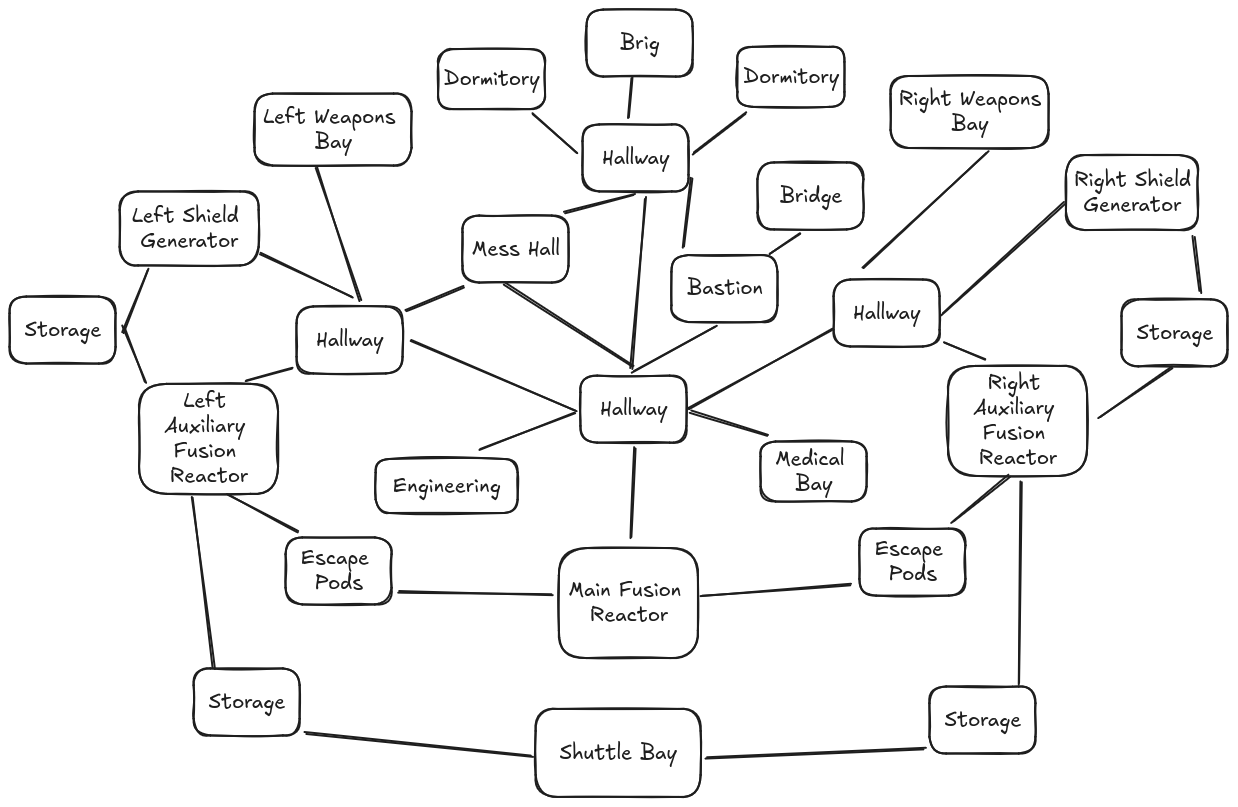
\includegraphics[width=.9\linewidth]{images/Space Ship.png}
\end{center}
\subsubsection{Weapons Bays}
\label{sec:org657558b}
Ships Values
\begin{itemize}
\item Attack 120
\item Defense 0
\item Power Consuption 60
\item Hull 75

\item 6 Enineers (CR 4)
\begin{itemize}
\item \aspect{Plasma Pistol 2}
\end{itemize}
\item \aspect{Danger: Explosive 5}
\item \aspect{Many nooks and crannies 4}
\end{itemize}
\subsubsection{Shield  Generators}
\label{sec:org68dc602}
Ships Values
\begin{itemize}
\item Attack 0
\item Defense 120
\item Power Consuption 180
\item Hull 50

\item 3 Enineers (CR 4)
\begin{itemize}
\item \aspect{Plasma Pistol 2}
\end{itemize}
\item \aspect{High Power Consuption 5}
\item \aspect{Many nooks and crannies 4}
\end{itemize}
\subsubsection{Auxiliary Fusion Reactors}
\label{sec:orgfc1317e}
Ships Values
\begin{itemize}
\item Attack 0
\item Defense 0
\item Power Consuption 180
\item Hull 50

\item 4 Enineers (CR 4)
\begin{itemize}
\item \aspect{Plasma Pistol 2}
\end{itemize}
\item 2 Guards (CR 5)
\begin{itemize}
\item \aspect{Plasma Rifle 3}
\end{itemize}
\item \aspect{High Power Consuption 5}
\end{itemize}
\subsubsection{Fusion Ractors}
\label{sec:org0bac500}
Ships Values
\begin{itemize}
\item Attack 0
\item Defense 0
\item Power Consuption 300
\item Hull 75

\item 4 Enineers (CR 4)
\begin{itemize}
\item \aspect{Plasma Pistol 2}
\end{itemize}
\item 4 Guards (CR 5)
\begin{itemize}
\item \aspect{Plasma Rifle 3}
\end{itemize}
\item \aspect{High Power Consuption 8}
\end{itemize}
\subsubsection{Brig}
\label{sec:orga11779f}
Ships Values
\begin{itemize}
\item Hull 50

\item One Guard (CR 5)
\begin{itemize}
\item Will use first round to raise the Alarm
\item \aspect{Plasma Rifle 3}
\end{itemize}
\item 5 Cells
\begin{itemize}
\item \aspect{Cell door 10[5]}
\end{itemize}
\item 3 Prisoners (each CR 3)
\end{itemize}
\subsubsection{Bridge}
\label{sec:org5d2d441}
Ships Values
\begin{itemize}
\item Hull 150

\item 1 Captain (CR 7)
\item 4 Officers (CR 6)
\begin{itemize}
\item \aspect{Plasma Pistol 2}
\end{itemize}
\item 2 Guards (CR 5)
\begin{itemize}
\item \aspect{Plasma Rifle 3}
\end{itemize}
\item \aspect{Lots of Computers 5}
\item can shut of any other rooms functions
\end{itemize}
\subsubsection{Bastion}
\label{sec:org50d9252}
Ships Values
\begin{itemize}
\item Hull 50

\item 1 Officers (CR 6)
\begin{itemize}
\item \aspect{Plasma Rifle 3}
\end{itemize}
\item 4 Guards (CR 5)
\begin{itemize}
\item \aspect{Plasma Rifle 3}
\end{itemize}
\item \aspect{Autoturret 12 [3]}
\item \aspect{Blast door 30 [5]}
\end{itemize}
\subsubsection{Mess Hall}
\label{sec:orgfb89b3f}
Ships Values
\begin{itemize}
\item Hull 50
\end{itemize}

During the first 3 Scenes, will some of the board personal be here. They will stow away all movable objects in the hall. Afterwards they will move to the shuttle bay in order to be ready for an evacuation.

\begin{itemize}
\item \aspect{}
\item 5 Ship Personel (CR 3)
\end{itemize}
\subsubsection{Medical Bay}
\label{sec:orgfcf1e0a}
Ships Values
\begin{itemize}
\item Hull 100
\end{itemize}

Whenever a room gets hit and destroyed some of the personel may be injured and brought to the medical bay. 

\begin{itemize}
\item 2 Docktors (CR 3)
\begin{itemize}
\item \apsect{Medical Training 4}
\item \apsect{Pacifist 2}
\end{itemize}
\item \aspect{Medical Equipment 6}
\end{itemize}
\section{One Shot: In the Necromancers Dungeon}
\label{sec:org82e0e1d}

A Medieval Fantasy scenario.

Escape from the dungeon of a necromancer.

The players play a group of people who were captured by a powerfull necromancer. The necromancer has conquered a small kingdom with his forces and regularly gets deliveries of prisoners which he uses for his necromantic experiments. The group find themselves in the dungeon cells. And need to flee. Through another half dead prisoner they get the information that escape is impossible. Every prisoner is magically marked and can always be found by the necromancers forces. The Necromancer is Arrogant and Cruel. If you can escape your only chance is defeating the necromancer and freeing this land from his scurge.  
\subsection{Cast}
\label{sec:org0d25b6b}

\begin{npc}{Knight}{at}{6 5 5 3 3 3 5 5}{54}
Aspects:
\begin{itemize}
\item Experieced Turney Combatant 5
\item Member of a noble family 4
\end{itemize}

\columnbreak

Traits:
\begin{itemize}
\item none
\end{itemize}
\end{npc}

\begin{npc}{Thief}{at}{5 7 3 4 3 5 3 3}{69}
Aspects:
\begin{itemize}
\item Member of the Shadows (thiefes guild) 5
\item Great free climber 3
\item Smooth talker 1
\end{itemize}

\columnbreak

Traits:
\begin{itemize}
\item Sink into Shadows
\end{itemize}
\end{npc}

\begin{npc}{Druid}{at}{3 3 5 6 3 3 5 5}{96}
Aspects:
\begin{itemize}
\item Circle of the eternal forrest druid 6
\item Herbalist 5
\item Recluse 2
\end{itemize}

\columnbreak

Traits:
\begin{itemize}
\item Protector and Servant of Nature
\end{itemize}
\end{npc}
\subsection{NPCs}
\label{sec:orgccbd361}

\begin{npc}{Necromancer}{at}{12 12 24 24 16 20 16 16}{264}
Aspects:
\begin{itemize}
\item Master of the Dark Arts 12
\item Divinator 10
\item Ruler of the Darklands 7
\item Sadistic Master of Pain 5
\item Shure of himself / Arrogant 5
\end{itemize}

\columnbreak

Traits:
\begin{itemize}
\item Lich
\item Necromantic Fleshweaver
\end{itemize}

Items:
\begin{itemize}
\item Skeleton Staff 6
\item Dagger of Pain 6
\end{itemize}
\end{npc}

\begin{npc}{Guard}{at}{4 4 3 3 3 3 3 3}{0}
Aspects:
\begin{itemize}
\item Trained Guard 3
\item Likes to Drink 2
\item 
\end{itemize}

\columnbreak

Traits:
\begin{itemize}
\item 
\end{itemize}
\end{npc}

\begin{npc}{Undead Abomination}{at}{6 6 1 1 1 1 0 0}{15}
Aspects:
\begin{itemize}
\item Hates life 6
\end{itemize}

\columnbreak

Traits:
\begin{itemize}
\item Undead
\item Obedient Servant
\end{itemize}
\end{npc}
\subsection{Map}
\label{sec:org01840f2}

\subsubsection{Dungeon (-1 floor)}
\label{sec:org85de5c6}
CR +0

The dungeon is a couple of hallways which are lined with small cells. Each cell has walls made from mordared rough stone and are shut with a metal banded heavy wooden door. The only sources of light are a dimmly glowing lichen and some magical candles in the hallways which are made from fingerbones.

\begin{itemize}
\item Very dim light 3
\item Rot and decay 3
\item Water dripping from the ceiling 2
\item Heavy iron banded doors
\end{itemize}
\subsubsection{Torture Chamber (-1 floor)}
\label{sec:org9833740}
CR +1

The pain and suffering of sentients are a powerfull ingredient if extracted correctly. The torture chamber has all the tools of the trade. Its ceiling is adorned by a green eye which appears to be unmoving yet always gives the eary feeling it is looking right at you. The eye extacts the pain and channels it into the green elixir which has to be placed on the altar on the far side if the room.

\begin{itemize}
\item all sorts of torture implements 6
\item 
\end{itemize}
\subsubsection{Pantry and Wine Cellar (-1 floor)}
\label{sec:org540eb1d}
CR -1

A long line of barrels line one side of this hallway. The other is lined with dusty wine bottles. To keep his mortal servants from stealing from his precious collection the necromancer has created the stalker. A scarily deformed skeleton whichis supposed to hide in the shadows and ambush and thiev. however it did sucumb to decay and now some of the guards steal a little from time to time.

\begin{itemize}
\item Dark nooks and crannies 4
\item Great wine 6
\item Vial of konzentrated suffering
\end{itemize}
\subsubsection{Necromantic Lab (-1 floor)}
\label{sec:org19afacc}
CR +2

In this horrid room full of horrors and half fished experiments. This is where all the necromancers special troops are stitched together. The players will find here some of the notes ot the dark mage, dangerous creatures and more than enough reason to hate. The partially build creatures here will attack the players once they come close enough.

\begin{itemize}
\item 
\end{itemize}
\subsubsection{Watch Room (0 floor)}
\label{sec:org179de58}
CR +2

A few bunk beds, a table, and some chairs are in this room, This is where the guards stay if they dont have to do their rounds. Most of the time there is at least one guard here. Either sleeping or playing cards at the table. Maybe even drinking some stolen wine.

\begin{itemize}
\item Well lit 2
\item Kind of chaotic 2
\item 
\end{itemize}
\subsubsection{Entrance Hall (0 floor)}
\label{sec:org138bf4f}
CR -2

The tall double winged door is closed. Outside, infront of the door stand a couple of heavyly armored guards.
\subsubsection{Alchemy Lab (0 floor)}
\label{sec:org153dce7}
CR +0

\begin{itemize}
\item All sorts of Alchemical instruments and ingredients 6
\item 
\end{itemize}
\subsubsection{Kitchen (0 floor)}
\label{sec:orge46029f}
CR +0

\begin{itemize}
\item Pots Pans and Knives 3
\end{itemize}
\subsubsection{Guest Rooms (1 floor)}
\label{sec:org31c2261}
CR +0
\subsubsection{Dining Room (1 floor)}
\label{sec:orgd01d382}
CR +0

A long table, made from Mahogany, is the centerpiece of this room. Despite the sice, and Luxury of this room, is it mainly used by the dark lord of this house to demonstrate his superiority.

\begin{itemize}
\item lucurious 5
\end{itemize}
\subsubsection{Living Chambers (2 floor)}
\label{sec:orgcba5741}
CR +2

The personal chambers of the lord are surprisingly simple, yet or of high qualit. The players have to be carefull as these rooms is always guarded. 

\begin{itemize}
\item Simple 3
\item Quality 3
\end{itemize}
\subsubsection{Library (3 floor)}
\label{sec:org6aa93b0}
CR +3

This room is frequently visited and occupied by the mage.

\begin{itemize}
\item A vast coleection of tomes 6
\end{itemize}
\subsubsection{Observatory (4 floor)}
\label{sec:org09c9811}
CR +4

On the very top of the tower and surounded by a balcony is the mages observagory.

\begin{itemize}
\item Tools of astronomy and divination 6
\end{itemize}
. High up 6
\section{One Shot: A night at the Hospital}
\label{sec:org69c0400}

A modern horror scenario.

The year is 1980. You play a group of collegue students who decided on a dare to spend a night in an abandoned hospital. Originally you came with more people but because of a stupid fight you split up into two groups. You settled down in one of the old patients rooms on the first floor. As the clock shows midnight, you hear a sudden bang, as all doors and windows of the hospital shut at once. From this point on they can not be opened by any means. You have to figure out how to escape from this situation. 

Background:
\begin{itemize}
\item The hospital has a very long history.
\begin{itemize}
\item The oldest part of the hospital is build in a former prison.
\item It was once a mental istitution.
\item A couple of years ago, there was a scandal when a nurse turned serial child murderer.
\end{itemize}
\item It is inhabited by several ghosts. Each has different goals.
\begin{itemize}
\item A ghost can be pacified or destroyed. For both you need an understanding of his history.
\end{itemize}
\end{itemize}
\subsection{Cast}
\label{sec:org1c2e1ce}

\subsubsection{History Student}
\label{sec:org61a9884}

\begin{npc}{History Student}{at}{4 3 2 3 4 2 3 3}{36}
Aspects:
\begin{itemize}
\item \aspect{History Nerd 3}
\item \aspect{Tourist Guide 1}
\item \aspect{Plays Sports 2}
\end{itemize}
\columnbreak

Traits:
\begin{itemize}
\item None
\end{itemize}

Items:
\begin{itemize}
\item Flashlight 1
\item Lighter 1
\end{itemize}
\end{npc}
\subsubsection{Linguistics Student}
\label{sec:org6325f6f}

\begin{npc}{Linguistics Student}{at}{3 2 3 4 3 3 3 3}{36}
Aspects:
\begin{itemize}
\item \aspect{Latin Nerd 3}
\item \aspect{Works in a Library 1}
\item \aspect{Plays the Guitar 2}
\end{itemize}
\columnbreak

Traits:
\begin{itemize}
\item None
\end{itemize}

Items:
\begin{itemize}
\item Flashlight 1
\item Guitar 2
\end{itemize}
\end{npc}
\subsubsection{Engineering Student}
\label{sec:org610a2a4}

\begin{npc}{Engineering Student}{at}{4 3 3 3 3 2 4 3}{30}
Aspects:
\begin{itemize}
\item \aspect{Engineer 3}
\item \aspect{Hobby car mechanic 2}
\end{itemize}
\columnbreak

Traits:
\begin{itemize}
\item None
\end{itemize}

Items:
\begin{itemize}
\item Flashlight 1
\item Pocketknive 2
\item Gaffa Tape 1
\end{itemize}
\end{npc}
\subsubsection{Phychology Student}
\label{sec:org3e62796}

\begin{npc}{Phychology Student}{at}{2 3 3 3 4 4 2 3}{36}
Aspects:
\begin{itemize}
\item \aspect{Phychology 3}
\item \aspect{Barista 1}
\item \aspect{Dancer 2}
\end{itemize}
\columnbreak

Traits:
\begin{itemize}
\item None
\end{itemize}

Items:
\begin{itemize}
\item Flashlight 1
\item Dance Shoes 1
\end{itemize}
\end{npc}
\subsubsection{Chemistry Student}
\label{sec:org5096f50}

\begin{npc}{Chemistry Student}{at}{3 3 2 5 2 2 4 3}{36}
Aspects:
\begin{itemize}
\item \aspect{Chemistry 3}
\item \aspect{Plays the Harmonica 1}
\item \aspect{Runner 2}
\end{itemize}
\columnbreak

Traits:
\begin{itemize}
\item None
\end{itemize}

Items:
\begin{itemize}
\item Flashlight 1
\item Chocolate Bar
\item Harmonica 1
\end{itemize}
\end{npc}
\subsection{NPCs}
\label{sec:org652de5e}


\begin{npc}{Mad Maggie the Child Murderer}{at}{3 3 2 5 2 2 4 3}{36}
Aspects:
\begin{itemize}
\item \aspect{Chemistry 3}
\item \aspect{Plays the Harmonica 1}
\item \aspect{Runner 2}
\end{itemize}
\columnbreak

Traits:
\begin{itemize}
\item None
\end{itemize}

Items:
\begin{itemize}
\item Flashlight 1
\item Chocolate Bar
\item Harmonica 1
\end{itemize}
\end{npc}

Maggie the Child Murderer

Dr. Francis Budgelburry the Famous Neurologist
\subsection{Rules}
\label{sec:org6d96629}

The ghosts are bound to the hospital in general and to their area in particular. They are able to move away from it but tend to avoid it out of habit.

The players are not able to leave the hospital in any way until they have dealt with the two ghosts.
\subsection{Map}
\label{sec:orgaab616f}

\subsubsection{Pharmacy (1 Floor)}
\label{sec:org137dc47}

Stalked by the shadows. If one of the shadows catches you it will try to carry you off into the Orthopedic ward. There they will Break your limbs.

Points of Interrest:
\begin{itemize}
\item You can find beta-blockers to calm your nerves.
\item You can find Koffein to stay awake.
\end{itemize}
\subsubsection{Kitchen (1 floor)}
\label{sec:org1c12ffe}

The kitchen is pure chaos. A bunch of poltergeists throw stuff around in here. Only the cleaning closet is untuched by the poltergeist.

\begin{itemize}
\item \aspect{Poltergeist 4}
\item \aspect{Save but insanely cold walk in fridge 5}
\end{itemize}

Points of Interrest:
\begin{itemize}
\item You can find some cooking oil from which you can make fuel for the ambulance.
\item You can find ingredients in the cleaning closet (the only)
\end{itemize}
\subsubsection{Outpatient and Atenual Ward (1 floor)}
\label{sec:orgddb7055}

Stalked by the shadows. If one of the shadows catches you it will try to carry you off into the Orthopedic ward. There they will Break your limbs.

Shadow (C 4):
\begin{itemize}
\item \aspect{Strong 8}
\item \aspect{Pushed away by light 3}
\item Incorporal and immportal
\end{itemize}
\subsubsection{Accident \& Emergency (1 floor)}
\label{sec:org21363d8}

If the players find the ambulance in the garage, they can try to bring it back to working condition. For this they need to repair the vehicle and get some fuel.

\begin{itemize}
\item \aspect{broken Ambulance 6}
\end{itemize}

Points of Interrest:
\begin{itemize}
\item You can find some tools here. \aspect{Hammers 1}, \aspect{Saws 2}. In one of the ambulances even a \aspect{crowbar 2}
\item You can find a pair of walky talkies here.
\end{itemize}
\subsubsection{Entrance Hall (1 floor)}
\label{sec:orgd35af0c}

The entrance hall is mostly like the players remember from when they came in. Since it is the way to everything else you can hear noised and feel winds comming from everywhere.

\begin{itemize}
\item \aspect{A feeling of strong unease and damger 2}
\end{itemize}


Points of Interrest:
\begin{itemize}
\item A brief history of the Hospital with maps and fotos.
\begin{itemize}
\item If looked at closely you can find a weird spot on the basements map from back in asylum times.
If cross referenced with the maps from prison times your find the spot of a hidden room. Today it borders on the Autopsy chambers.
\end{itemize}
\end{itemize}
\subsubsection{Fracture/Orthopedic Clinic (2 floor)}
\label{sec:orgf631ee2}

Stalked by the shadows. If one of the shadows catches you it will try to carry you off into the Orthopedic ward. There they will Break your limbs.
\subsubsection{Surgery theathres (2 floor)}
\label{sec:org0f80a13}
The former surgery theatres and neighboring rooms smell weird. Sometimes a fog moves through the rooms. If a creature is caught in it it tends to put them to sleep.

\begin{itemize}
\item \aspect{The smell of pain 3}
\item \aspect{Anestetic Fog 4}
\end{itemize}

Points of Interrest:
\begin{itemize}
\item A display cabinet with the original notebook of a famous neurologist (TODO Name) who worked here back when it was an insame asylum.
\begin{itemize}
\item If read by the players they can find notes about operations on patient during which he found several abnormalities with their brains.
\item If cross referenced with the notes you can find in administration you will find out that those patiens where officially not operated on but died by other causes just before the date of the operation.
\item You can find a hint on where in the basement the operation room should be.
\end{itemize}
\end{itemize}
\subsubsection{Chapel (2 floor)}
\label{sec:orgbf94dd9}

\begin{itemize}
\item \aspect{Sancutary for the Believers 4}
\end{itemize}
\subsubsection{Administration (3 floor)}
\label{sec:orgb302ad3}

\begin{itemize}
\item \aspect{Chaos 3}
\end{itemize}

Points of Interrest:
\begin{itemize}
\item If you go through the notes you may find:
\begin{itemize}
\item Asylum Patient Records: It contains lists of patients, their arrival, conditions and release or death date. Also the cause of death if applicable. If cross referenced with the notebook from the Surgery Theatre then \ldots{} (see there)
\item Personel Records: If they search for the Murderous Nurse then they will find out that her grandmother died in the insame asylum. If they search for her in asylum records then they will find how she had murderous rages whenever she was separated from her Baby Blanket. Beacuse of company policy it was once taken from her completely and put into storage.
\end{itemize}
\end{itemize}
\subsubsection{Pediadric and Maternity Ward (3 floor)}
\label{sec:org40425c4}

The pediatric ward is stalek by the ghost of the Murderous Nurse. She stalks through the rooms hunting the ghosts of the children. If a player is seen by her then she will hunt them. She is corporeal and will react to being fought with weapons. But she can not die. If she is slain her body will disintegrate and she will soon stalk the halls again.

\begin{itemize}
\item \aspect{Childrens Noises 2}
\end{itemize}

Mad Maggie (C 4xPlayers):
\begin{itemize}
\item \aspect{Murderous 6}
\item \aspect{Terrifying 6}
\item \aspect{Sadistic 6}
\item \aspect{Impulsive 6}
\item \aspect{Broken Mind of a Mad Woman 6}
\end{itemize}
\subsubsection{Autopsie (-1 floor)}
\label{sec:org7b50521}
Set in a renovated part of the former Prison Celar is the autopsy department. The main room is lined with a wall of body storages.
When the group comes into the room the dead in the storages begin to rise. They start to move and pound on the doors. If freed or if they had enough time to free selselves they will fight the living. Once the dead have left their confinement the lights turn of and only blink for a second when turned on again. Flashlights may still work normally.

\begin{itemize}
\item \aspect{Unnaturally Cold 3}
\item \aspect{Sharp Instruments 4}
\item \aspect{Lights out 4}
\end{itemize}

Zombie (C 3)
\begin{itemize}
\item \aspect{Unnaturally strong 2}
\item \aspect{Unfeeling undead 2}
\item \aspect{Literally Brainless 3}
\end{itemize}

Points of Interrest:
\begin{itemize}
\item The zombies are the patients of the famous nuerologist. They all have some mark of surgery on their heads.
\item Entrance to secret surgery room: Behind the wall where the bodys are stored there is the old surgery room of the neurologist. This can be found out in the entrance hall.
\end{itemize}
\subsubsection{storage cellar (-1 floor)}
\label{sec:org0f9bcae}
Since the Hospital is build on a former Prison its cellar still has that layout. The rooms are fillesd.

\begin{itemize}
\item \aspect{Prison Doors 3 [10]}
\item \aspect{A bunch of Random Stuff in Storage 5}
\item \aspect{Flickering Lights 2}
\end{itemize}

Points of Interrest:
\begin{itemize}
\item In a few of the rooms you can find a bunch of very old numbered boxes. In them is very random stuff.
\begin{itemize}
\item One of the boxes contains the baby blanket of the murderous nurses grandmother. This can be used to pacify the ghost.
\end{itemize}
\end{itemize}


\newpage
\thispagestyle{empty}

\begin{center}
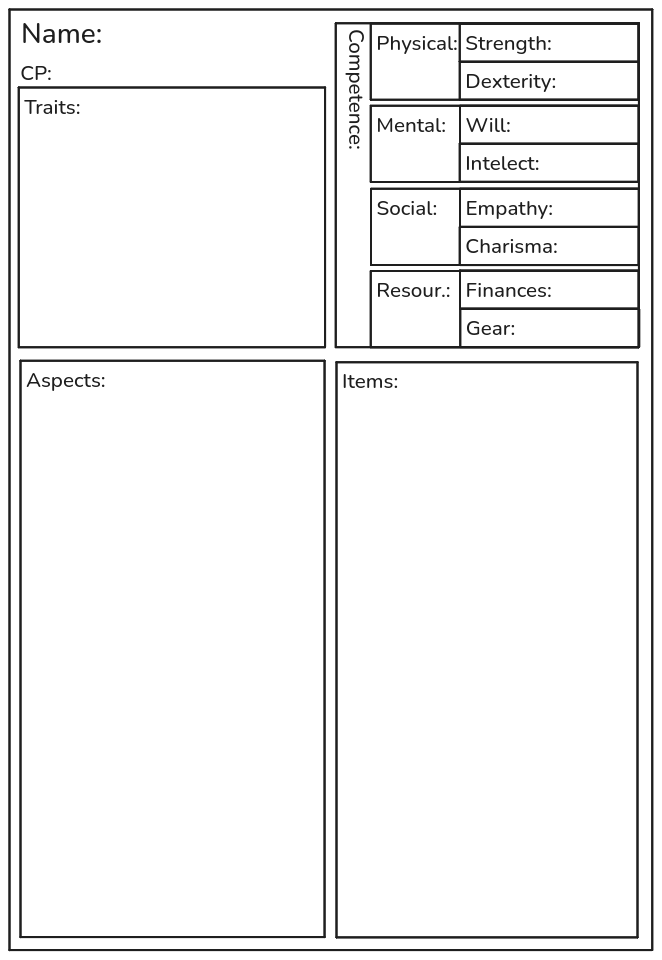
\includegraphics[width=1.0\textwidth]{images/Character Sheet.png}
\end{center}

\setlength{\hoffset}{0pt}
\setlength{\voffset}{0pt}
\setlength{\textwidth}{14cm}
\end{document}
